\hypertarget{a00354}{}\section{Linked parameters}
\label{a00354}\index{Linked parameters@{Linked parameters}}
How to link parameters. 

\hypertarget{a00354_linkedParameters_contents}{}\subsection{On this page}\label{a00354_linkedParameters_contents}
\begin{DoxyItemize}
\item \hyperlink{a00354_linkedParameters_basics}{Basics of Linked Parameters} \item \hyperlink{a00354_linkedParameters_linkedParameterOperation}{Linked Parameter Operation} \item \hyperlink{a00354_linkedParameters_changingTapers}{Changing Tapers}\end{DoxyItemize}
\hypertarget{a00354_linkedParameters_basics}{}\subsection{Basics of Linked Parameters}\label{a00354_linkedParameters_basics}
A \char`\"{}linked\char`\"{} parameter can be defined as any parameter whose state is somehow dependent on another parameter. Within this general definition, there are various different kinds of parameter linking\+:


\begin{DoxyItemize}
\item Linking behavior can operate one-\/way or parameters can be reciprocally linked
\item Linking between parameters can be one-\/to-\/one or one-\/to-\/many
\end{DoxyItemize}\hypertarget{a00354_linkedParameters_considerations}{}\subsubsection{Basic considerations for parameter linking}\label{a00354_linkedParameters_considerations}
Although the concept of parameter linking is simple, implementing linked parameter behavior that is intuitive and consistent can require careful design.


\begin{DoxyItemize}
\item Parameter interdependencies and constraints can become complex, especially when handling multiple sets of linked parameters.
\item Linked parameters that update other parameters during playback can result in subtle timing inconsistencies
\item Automated parameters may contain arbitrary and conflicting automation data
\item A user may attempt to edit multiple linked parameters simultaneously during playback, e.\+g. using multiple encoders on a control surface
\item A plug-\/in may contain dependency cycles between interdependent parameters. These cycles can cause undesired behavior that is difficult to debug, especially if it only occurs in certain circumstances such as when loading particular presets.
\end{DoxyItemize}

In all of these cases, a plug-\/in should provide consistent linked parameter behavior\+: every automated playback pass should be identical, parameters should never \char`\"{}fight\char`\"{} one another or trigger rapid and unexpected changes in other parameters, parameters should not become \char`\"{}stuck\char`\"{} in a particular state, etc.

 Here comes trouble\hypertarget{a00354_linkedParameters_behavior}{}\subsubsection{Defining proper linked parameter behavior}\label{a00354_linkedParameters_behavior}
A good way to approach parameter linking is to start with an understanding of exactly what behavior you desire.

Here are some behaviors that you probably {\itshape don\textquotesingle{}t} want in your plug-\/in\+:


\begin{DoxyItemize}
\item B\+A\+D\+: Parameters are only linked when edited from the plug-\/in G\+U\+I  Users may attempt to edit linked parameters from attached control surfaces or using the host\textquotesingle{}s automation features. The parameters should behave the same way regardless of which method is used to edit them.  
\item B\+A\+D\+: Parameters try to match all automation data  Automation data can be written arbitrarily\+: Pro Tools doesn\textquotesingle{}t have any restrictions that a user with a pencil tool must draw inside the lines, or a user may attempt to edit multiple parameters on an attached control surface simultaneously. Any parameter that attempts to match both its own automation data and the automation data of another parameter, or any parameter that attempts to set another automatable parameter\textquotesingle{}s state based on its own automation data, will lead to \char`\"{}fighting\char`\"{} during playback of non-\/conformant automation.  
\item B\+A\+D\+: Automation data is only written to one lane at a time  One approach to parameter linking may be to only write automation data to a single parameter at a time. This could be the parameter that is currently being touched and edited, or it could be a dedicated \char`\"{}master\char`\"{} parameter within the linked group. While this approach can be used to solve some types of conflicts, it can still lead to unnecessarily complex or inconsistent behavior in certain situations\+: for example, arbitrary automation data can still be written to multiple parameters\textquotesingle{} automation lanes, or a user can choose to record automation for only one parameter in a set but can skip the \char`\"{}master\char`\"{} parameter. Furthermore, it is difficult if not impossible to properly handle parameters that can be dynamically linked or un-\/linked using this approach.  
\end{DoxyItemize}

With those potential problems in mind, here is a description of how parameter linking {\itshape should} behave.\hypertarget{a00354_linkedParamters_behavior_correct}{}\paragraph{Correct behavior for linked parameters}\label{a00354_linkedParamters_behavior_correct}
{\itshape Notes}
\begin{DoxyItemize}
\item In this proposal (and throughout the rest of this page) the term \char`\"{}linker\char`\"{} will refer to a parameter that initiates a change and the term \char`\"{}linked\char`\"{} will refer to a dependent parameter that receives the change.
\item The following discussion will focus on {\itshape automatable} parameters that are {\itshape reciprocally linked}. This case tends to be the most complex, with the greatest need for consistency of implementation.
\end{DoxyItemize}

{\itshape During user-\/generated real-\/time edits} (from the plug-\/in G\+U\+I or a control surface) both the linker and the linked parameters should be updated. Without this requirement, there would be no parameter linking. In order for this requirement to be enforced consistently the following behaviors must be maintained\+: 
\begin{DoxyItemize}
\item The linked parameter should not jump to a new value if the user attempts to edit both parameters simultaneously using a control surface.  
\item To ensure proper automation playback, automation should be written to both the linker and the linked parameters.  
\end{DoxyItemize}

{\itshape When playing back automation}, parameters should operate independently and should not attempt to force dependent parameters to a new state. This prevents fighting in the presence of incompatible automation and ensures deterministic automation playback with every playback pass. As above, there are some more subtle behaviors that must be maintained for this to work properly\+: 
\begin{DoxyItemize}
\item If the user begins a real-\/time edit during automation playback then the parameter linking behavior should resume as described above  
\item If the plug-\/in\textquotesingle{}s algorithm cannot support certain parameter configurations then its automatable parameters should be decoupled from the algorithm using a set of coefficients that is aware of the algorithm\textquotesingle{}s constraints. In this way every combination of parameter states can map to a particular coefficient state, maintaining determinism, and incompatible parameter combinations can simply resolve to the \char`\"{}closest\char`\"{} match in the possible coefficient space during playback of edited parameter automation data. 
\item Another, simpler approach for plug-\/ins that do not support arbitrary parameter configurations is to ensure that the problematic parameters are not automatable. Handling non-\/automatable parameter linking is much easier in general, so consider this approach if automation is not a requirement for some of your plug-\/in\textquotesingle{}s parameters.  
\end{DoxyItemize}

{\itshape When handling preset changes and plug-\/in initialization}, a similar approach should be taken as with plug-\/in automation playback. In these cases it is very unlikely that the plug-\/in\textquotesingle{}s parameters will be left in an incompatible state and attempts at linking may result in unwanted update cycles between inter-\/dependent parameters or unnecessary coefficient churn. This latter concern can be a real problem for A\+A\+X D\+S\+P plug-\/ins that initialize internal algorithmic state based on initial coefficient data.\hypertarget{a00354_linkedParamters_behavior_caveat}{}\paragraph{Compatibility caveat}\label{a00354_linkedParamters_behavior_caveat}
This behavior was not possible under the R\+T\+A\+S/\+T\+D\+M format, and many R\+T\+A\+S and T\+D\+M plug-\/ins reverted to workarounds such as writing automation to only one parameter at a time and linking the parameters during playback. Therefore, plug-\/ins that previously supported linked automatable parameters under the R\+T\+A\+S/\+T\+D\+M format may not be able to both implement this recommended parameter linking behavior and maintain compatibility with automation in saved sessions.

Most of Avid\textquotesingle{}s plug-\/ins that were available in the R\+T\+A\+S and T\+D\+M formats fall into this category and should not be used as examples of proper parameter linking behavior. Instead, use the S\+D\+K\textquotesingle{}s Demo\+Gain\+\_\+\+Linked\+Parameters example plug-\/in as an example of proper linked parameter operation.\hypertarget{a00354_linkedParameters_linkedParameterOperation}{}\subsection{Linked Parameter Operation}\label{a00354_linkedParameters_linkedParameterOperation}
As described above, the key rule for linked parameters is to link during real-\/time user edits {\itshape only}, and should operate the parameters independently (without linked behavior) during automation playback and preset restore. This rule will simplify many issues\+: it will prevent conflicts with automation data, avoid potentially strange behaviors when restoring presets, and more.

Here is how the system works W\+I\+T\+H linked parameters, using code snippets from the Demo\+Gain\+\_\+\+Linked\+Parameters example plug-\/in\+:\hypertarget{a00354_linkedParameters_linkedParameterOperation_userEditing}{}\subsubsection{User Editing}\label{a00354_linkedParameters_linkedParameterOperation_userEditing}

\begin{DoxyEnumerate}
\item User clicks on a parameter in the G\+U\+I or grabs a parameter on the controls surface. A T\+O\+U\+C\+H token should be sent at this point.
\begin{DoxyItemize}
\item The touched parameter status comes back to the plug-\/in. If the parameters are linked the other linked parameter should have a T\+O\+U\+C\+H token sent. This really should only be done for linked continuous parameters. This is done by overriding the \hyperlink{a00018_a1555fe9834764330bd264941a1d6ebc3}{A\+A\+X\+\_\+\+C\+Effect\+Parameters\+::\+Update\+Parameter\+Touch()} method.
\end{DoxyItemize}
\item The user changes the parameter from the G\+U\+I or controls surface. A S\+E\+T token should be sent at this point. 
\begin{DoxyCode}
\textcolor{comment}{// *******************************************************************************}
\textcolor{comment}{// METHOD:  UpdateParameterTouch}
\textcolor{comment}{// *******************************************************************************}
\hyperlink{a00149_a4d8f69a697df7f70c3a8e9b8ee130d2f}{AAX\_Result} DemoGain\_Parameters::UpdateParameterTouch ( \hyperlink{a00149_a1440c756fe5cb158b78193b2fc1780d1}{AAX\_CParamID} inParameterID, 
      \hyperlink{a00149_aa216506530f1d19a2965931ced2b274b}{AAX\_CBoolean} inTouchState )
\{
    \textcolor{keywordflow}{if} ( inTouchState )
    \{
        \hyperlink{a00149_a1440c756fe5cb158b78193b2fc1780d1}{AAX\_CParamID} linkedControl = this->GetLinkedControl ( inParameterID );
        \textcolor{keywordflow}{if} ( linkedControl )
        \{
            this->TouchParameter ( linkedControl );
            mLinkTouchMap.insert ( std::pair<std::string,std::string>( inParameterID, linkedControl ) );
        \}
    \}
    [...]
\}
\end{DoxyCode}

\item The S\+E\+T token goes into the system and comes back to the plugin via \hyperlink{a00018_a56a9f41a975b48f583655db7b43aae5a}{A\+A\+X\+\_\+\+C\+Effect\+Parameters\+::\+Update\+Parameter\+Normalized\+Value()}.
\begin{DoxyItemize}
\item If the parameter is linked then the other linked parameter should have its value set for its linked behaviour. The system knows this is a linked parameter so when the value comes back to the plug-\/in via Update\+Parameter\+Normalized\+Value() it will know not to perform linked behaviors on that value change. To determine if a parameter should set a linked parameter you check it with the \hyperlink{a00018_af5445bb9f40ccf826227199647e140ee}{A\+A\+X\+\_\+\+C\+Effect\+Parameters\+::\+Is\+Parameter\+Touched()} method.
\end{DoxyItemize}
\item The plug-\/in updates its internal state and sends an U\+P\+D\+A\+T\+E tokens for both parameters. 
\begin{DoxyCode}
\textcolor{comment}{// *******************************************************************************}
\textcolor{comment}{// METHOD:  UpdateParameterNormalizedValue}
\textcolor{comment}{// *******************************************************************************}
\hyperlink{a00149_a4d8f69a697df7f70c3a8e9b8ee130d2f}{AAX\_Result} DemoGain\_Parameters::UpdateParameterNormalizedValue ( 
      \hyperlink{a00149_a1440c756fe5cb158b78193b2fc1780d1}{AAX\_CParamID} inParameterID, \textcolor{keywordtype}{double} inValue, \hyperlink{a00206_a30be0398faf20c6b121239eb9399f3f7}{AAX\_EUpdateSource} inSource )
\{
    \hyperlink{a00149_a4d8f69a697df7f70c3a8e9b8ee130d2f}{AAX\_Result}    result = 
      \hyperlink{a00018_a56a9f41a975b48f583655db7b43aae5a}{AAX\_CEffectParameters::UpdateParameterNormalizedValue} 
      ( inParameterID, inValue, inSource );
    \textcolor{keywordtype}{bool}        touched = this->IsParameterTouched ( inParameterID );

    [...]
                \textcolor{keywordflow}{if} ( touched && inSource == \hyperlink{a00206_a30be0398faf20c6b121239eb9399f3f7aec16143f3916bad3c5a6d8eb60600a3b}{AAX\_eUpdateSource\_Unspecified} )
                \{
                    \textcolor{keywordflow}{if} ( type == eType\_Pan )
                        this->SetParameterNormalizedValue( linkedControl, (1.0 - inValue) );
                    \textcolor{keywordflow}{else} \textcolor{keywordflow}{if} ( type == eType\_Gain )
                        this->SetParameterNormalizedValue( linkedControl, inValue );
                \}
    [...]
\}
\end{DoxyCode}

\item Repeat steps 2-\/4 while changing the parameter.
\item The user lets go of the G\+U\+I or controls surface. A T\+O\+U\+C\+H token with the released state should be sent.
\begin{DoxyItemize}
\item The touched parameter status comes back to the plug-\/in. If the parameters were linked the other linked parameter should have a T\+O\+U\+C\+H token with the release status sent. This again is done by overriding the \hyperlink{a00018_a1555fe9834764330bd264941a1d6ebc3}{A\+A\+X\+\_\+\+C\+Effect\+Parameters\+::\+Update\+Parameter\+Touch()} method. 
\begin{DoxyCode}
\textcolor{comment}{// *******************************************************************************}
\textcolor{comment}{// METHOD:  UpdateParameterTouch}
\textcolor{comment}{// *******************************************************************************}
\hyperlink{a00149_a4d8f69a697df7f70c3a8e9b8ee130d2f}{AAX\_Result} DemoGain\_Parameters::UpdateParameterTouch ( \hyperlink{a00149_a1440c756fe5cb158b78193b2fc1780d1}{AAX\_CParamID} inParameterID, 
      \hyperlink{a00149_aa216506530f1d19a2965931ced2b274b}{AAX\_CBoolean} inTouchState )
\{
    \textcolor{keywordflow}{if} ( inTouchState )
    \{
        [...]
    \}
    \textcolor{keywordflow}{else}
    \{
        [...]
            this->ReleaseParameter ( iter->second.c\_str () );
        [...]
    \}

    \textcolor{keywordflow}{return} \hyperlink{a00207_a5f8c7439f3a706c4f8315a9609811937aeddbd1bb67e3a66e6af54a4b4a7a57b3}{AAX\_SUCCESS};
\}
\end{DoxyCode}

\end{DoxyItemize}
\end{DoxyEnumerate}\hypertarget{a00354_linkedParameters_linkedParameterOperation_automationPlayback}{}\subsubsection{Automation Playback}\label{a00354_linkedParameters_linkedParameterOperation_automationPlayback}

\begin{DoxyEnumerate}
\item The S\+E\+T token comes from the automation system and enters the plugin via \hyperlink{a00061_a685858711efb8634ce66c327f2865c71}{Update\+Parameter\+Normalized\+Value()}.
\begin{DoxyItemize}
\item The plug-\/in will know this is not from the user editing therefore it will N\+O\+T set the other linked parameter. Remember O\+N\+L\+Y L\+I\+N\+K U\+S\+E\+R E\+D\+I\+T\+I\+N\+G. That way there\textquotesingle{}s no conflicts if the user edited the automation or if the order in which automation arrives at the plug-\/in changes.
\end{DoxyItemize}
\item The plug-\/in updates its internal state and sends an U\+P\+D\+A\+T\+E token.
\item Repeat steps 1-\/2 while playing back automation.
\end{DoxyEnumerate}\hypertarget{a00354_linkedParameters_linkedParameterOperation_chunkRestoring}{}\subsubsection{Chunk Restoring}\label{a00354_linkedParameters_linkedParameterOperation_chunkRestoring}

\begin{DoxyEnumerate}
\item Plug-\/in loads the chuck.
\item The plug-\/in sets every parameters value.
\item The S\+E\+T tokens comes back to the plugin via Update\+Parameter\+Normalized\+Value().
\begin{DoxyItemize}
\item The plug-\/in will know this is not from the user editing therefore it will N\+O\+T set the other linked parameter. Remember O\+N\+L\+Y L\+I\+N\+K U\+S\+E\+R E\+D\+I\+T\+I\+N\+G. Hopefully the result of this is that the contents of the chunk will be restored to its exact state.
\end{DoxyItemize}
\item The plug-\/in updates its internal state and sends out U\+P\+D\+A\+T\+E tokens.
\end{DoxyEnumerate}\hypertarget{a00354_linkedParameters_changingTapers}{}\subsection{Changing Tapers}\label{a00354_linkedParameters_changingTapers}
One common use of linked parameters is to change the taper associated with a parameter. For changing tapers there are basically only a two rules you need to follow\+:


\begin{DoxyEnumerate}
\item When you\textquotesingle{}re loading a new chunk you need to set the taper values first. If a parameter is what updates the taper then set that value first. That way when the value of a parameter is set from a chunk it wont change because of a taper change.
\item Update the taper from the Update\+Parameter\+Normalized\+Value() method. If the new taper needs to change the value of the parameter you only do so if the user is editing the linked parameter. This still follows the O\+N\+L\+Y L\+I\+N\+K U\+S\+E\+R E\+D\+I\+T\+I\+N\+G rule.
\end{DoxyEnumerate}


\begin{DoxyCode}
\hyperlink{a00149_a4d8f69a697df7f70c3a8e9b8ee130d2f}{AAX\_Result} Simple\_Parameters::UpdateParameterNormalizedValue ( 
      \hyperlink{a00149_a1440c756fe5cb158b78193b2fc1780d1}{AAX\_CParamID} inParameterID, \textcolor{keywordtype}{double} inValue, \hyperlink{a00206_a30be0398faf20c6b121239eb9399f3f7}{AAX\_EUpdateSource} inSource )
\{
    \textcolor{comment}{// GetLinkedControl() is a user defined method which determines the linked control ID.}
    \hyperlink{a00149_a1440c756fe5cb158b78193b2fc1780d1}{AAX\_CParamID} linkedControl = this->GetLinkedControl ( inParameterID );
    \textcolor{keywordflow}{if} ( linkedControl )
    \{
        \textcolor{comment}{// IsParameterLinkReady()* is a built in method of AAX\_CEffectParameters which determines if the }
        \textcolor{comment}{// parameter should perform linked behaviors based on the touch state of the parameter and the }
        \textcolor{comment}{// source of the UpdateParameterNormalizedValue() call.}
        \textcolor{keywordflow}{if} ( this->IsParameterLinkReady ( inParameterID, inSource ) )
            this->SetParameterNormalizedValue( linkedControl, inValue );
    \}

    \textcolor{comment}{// Call the inherited method for the original parameter}
    \hyperlink{a00149_a4d8f69a697df7f70c3a8e9b8ee130d2f}{AAX\_Result}   result = 
      \hyperlink{a00018_a56a9f41a975b48f583655db7b43aae5a}{AAX\_CEffectParameters::UpdateParameterNormalizedValue} 
      ( inParameterID, inValue, inSource );
    \textcolor{keywordflow}{return} result;
\}
\end{DoxyCode}
 Collaboration diagram for Linked parameters\+:
\nopagebreak
\begin{figure}[H]
\begin{center}
\leavevmode
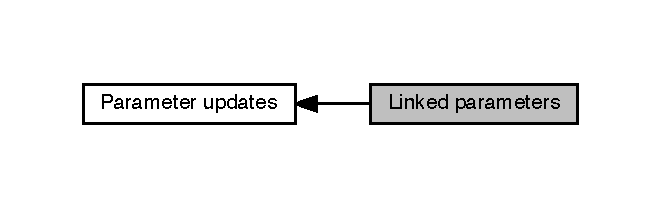
\includegraphics[width=317pt]{a00354}
\end{center}
\end{figure}
